\begin{figure}[H]
	\centering
	\footnotesize

	\psfrag{pde}[c][c] {$\text{PDE}$}
	\psfrag{eq}[c][c] {$\mathbf{\nabla}\cdot\textcolor[rgb]{0,0,1}{\mathbb{C}^{f^{Aloc}(\Omega)}}\mathbf{\nabla}^{(s)} \Bu + \rho \Bb = \Bf$}

	\psfrag{sgm}[c][c] {$\textcolor[rgb]{1,0.41,0.13}{\sigma_{ij}} = \textcolor[rgb]{0,0,1}{\mathbb{C}_{ijkl}^{f^{Aloc}(\Omega)}}\
		\textcolor[rgb]{0,0.4,0}{\varepsilon_{kl}}$}
	\psfrag{u}[c][c] {$\textcolor[rgb]{1,0,0}{u_{i}}$}
	\psfrag{eps}[c][c] {$\displaystyle \textcolor[rgb]{0,0.4,0}{\varepsilon_{ij}} 
	        = \frac{1}{2}\left(\textcolor[rgb]{1,0,0}{\partial_{j}u_{i}} +
			\textcolor[rgb]{1,0,0}{\partial_{i}u_{j}}\right)$}
	\psfrag{estr}[c][c] {$\displaystyle \textcolor[rgb]{0.5,0,0.5}{\mathcal{E}_{\text{strain}} }:=
		\frac{1}{2}\textcolor[rgb]{1,0.41,0.13}{\sigma_{ij}}\textcolor[rgb]{0,0.4,0}{\varepsilon_{ij}}$}

	\psfrag{ds}[l][l] {$\text{\scriptsize Displacement solution}$}
	\psfrag{stra}[l][l] {$\text{\scriptsize Infinitesimal strain}$}
	\psfrag{est}[l][l] {$\text{\scriptsize Cauchy Stress}$}
	\psfrag{js}[l][l] {$\text{\scriptsize Strain energy density }$}
	\psfrag{ljs}[l][l] {$\textsc{Strain energy density }$}
	\psfrag{gf}[l][l] {$\textsc{Griffith criterion}$}

	\psfrag{er}[l][l] {$\text{\scriptsize Energy}$}
	\psfrag{sfer}[l][l] {$\text{\scriptsize Crack-opening surface energy (COSE)}$}
	\psfrag{tser}[l][l] {$\text{\scriptsize Released strain energy (RSE)}$}
	\psfrag{tote}[l][l] {$\text{\scriptsize Total energy}$}
	\psfrag{crle}[l][l] {$\text{\scriptsize Virtual crack length}$}

	\psfrag{efcn}[l][l] {$\mathcal{E}(\Bx)$}
	\psfrag{fsf}[l][l] {$\mathcal{E}_{\text{COSE}}(\Bx)$}
	\psfrag{fse}[l][l] {$\mathcal{E}_{\text{RSE}}(\Bx)$}
	\psfrag{drf}[l][l] {$\mathcal{E}_{\text{RSE}}(\Bx) = \hat{f}(\Bx;\textcolor[rgb]{0.5,0,0.5}{\mathcal{E}_{\text{strain}}})$}
	\psfrag{etot}[l][l] {$\mathcal{E}_{\text{total}}(\Bx)$}

	\psfrag{nlt}[l][l] {$\mathcal{E}_{\text{total}}(\Bx)$}
	\psfrag{tnlt}[l][l] {$\mathcal{E}_{\text{total}}(\Bx) = \mathcal{E}_{\text{COSE}}(\Bx) + \mathcal{E}_{\text{RSE}}(\Bx)$}

	\psfrag{fet}[c][c] {$\mathcal{E}_{\text{total}}(\Bx) = \mathcal{E}_{\text{surface}} + \mathcal{E}_{\text{released strain}}$}
	\psfrag{ets}[l][l] {$\mathcal{E}_{\text{released strain}} = -\frac{\sigma^2}{2\BE}\pi a^2$}

	\psfrag{ac}[c][c] {$x_{\text{Griff}}$}
	\psfrag{x}[c][c] {$x$}
	\psfrag{y}[c][c] {$y$}
	\psfrag{bx}[c][c] {$\Bx$}

	\psfrag{Cm}[l][l] {$\textcolor[rgb]{0,0,1}{\mathbb{C}_{ijkl}^{f^{Aloc}(\Omega)}}$}

	\psfrag{oh}[c][c] {$O$}

	\psfrag{lf}[c][c] {$\bar{f}$}

	\psfrag{nd}[c][c] {$\text{Non-deformed}$}
	\psfrag{ud}[c][c] {$\text{Deformed}$}

	\psfrag{xnz}[c][c] {$\textcolor[rgb]{0.5,0,0.5}{\mathcal{E}_{\text{strain}}} = 0$}
	\psfrag{xns}[c][c] {$\textcolor[rgb]{0.5,0,0.5}{\mathcal{E}_{\text{strain}}} = \bar{\mathcal{E}}_{\text{strain}}$}
	\psfrag{xrl}[c][c] {$\mathcal{E}_{\text{RSE}}(\Bx) \propto \bar{\mathcal{E}}_{\text{strain}}$}

	\psfrag{frl}[c][c] {$O$}

	\psfrag{fx}[l][l] {$f(\Bx):= \mathcal{E}_{\text{total}}(\Bx) = \mathcal{E}_{\text{COSE}}(\Bx) + \mathcal{E}_{\text{RSE}}(\Bx)$}
	\psfrag{p}[l][l] {$\Bx_{\text{Griff}} = \Bx^* = \arg\displaystyle\ \max_{\Bx\in \mathbb{R}_{+}} f(\Bx)$}
	\psfrag{op}[l][l] {$\rightarrow \ \text{Optimization problem}$}

	\psfrag{fer}[c][c] {$[3]$}

	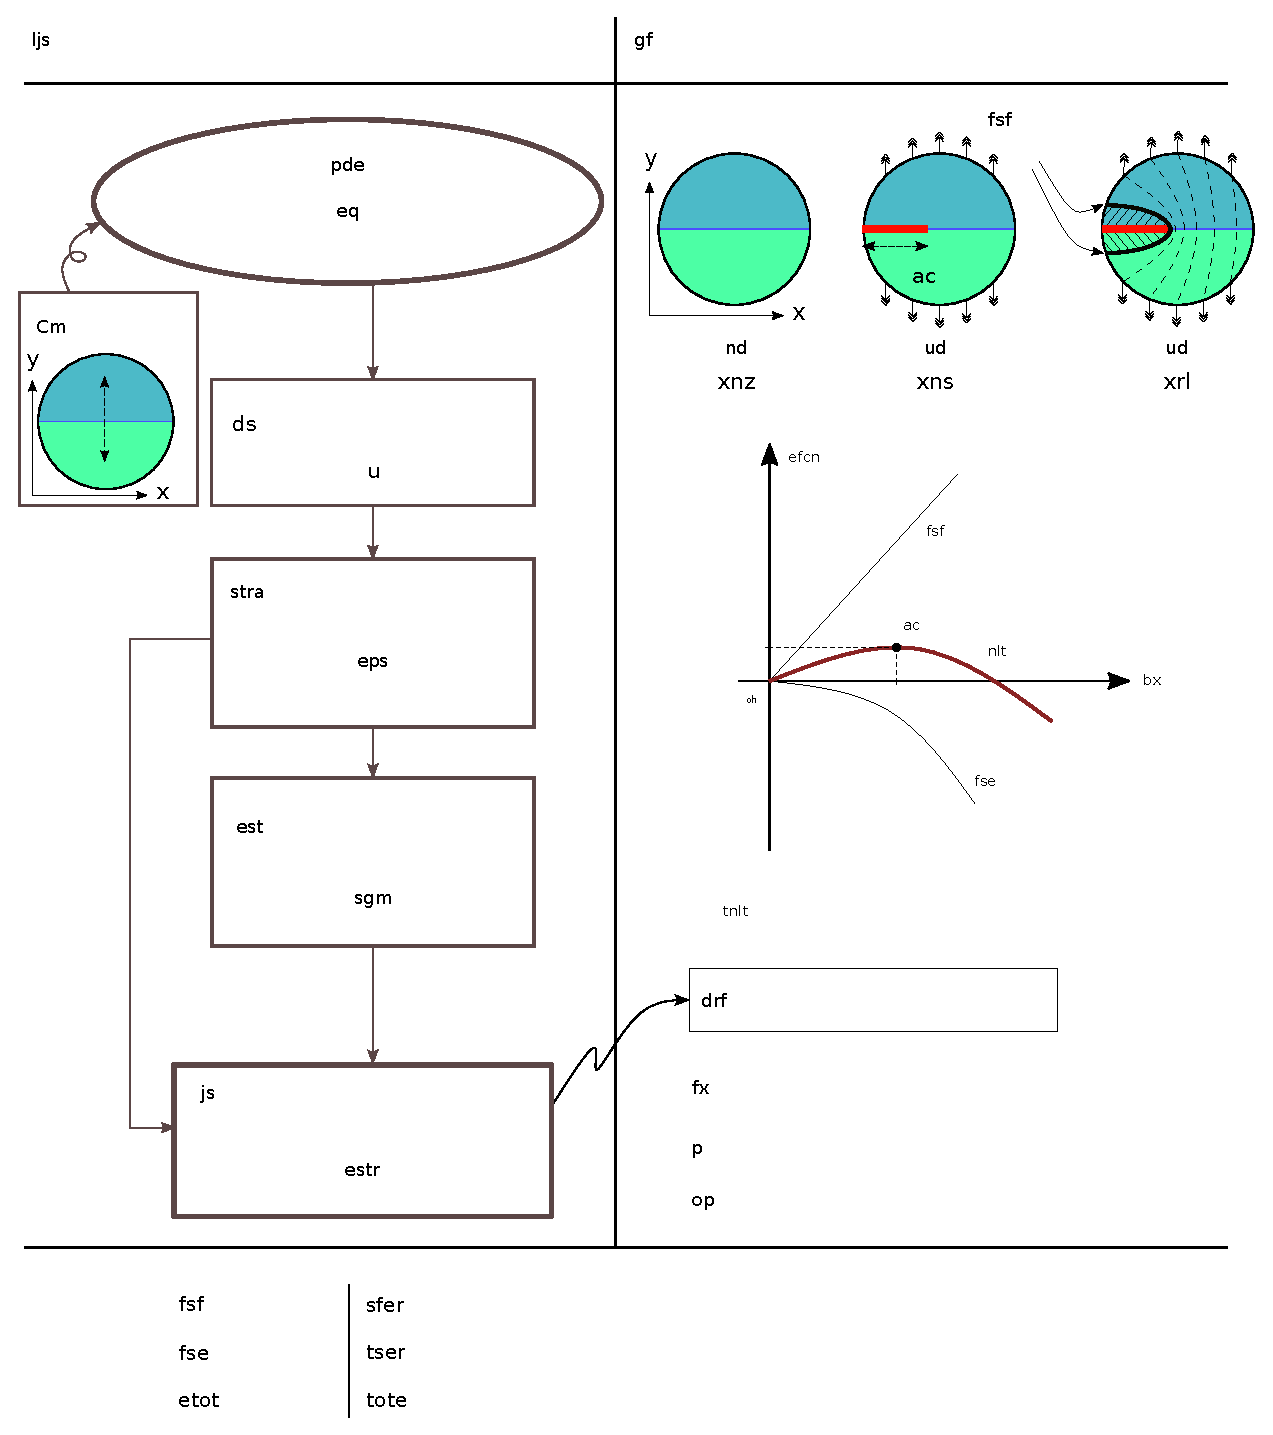
\includegraphics[width=1\textwidth]{griffith_flowchart_plus.eps}
	%\includegraphics[width=0.6\paperwidth]{fGaussLogistic_stress_cases.eps}
	\caption{Energy scale bridging and relative connection between strain energy density and Griffith criterion.}
	\label{\LABEL}
\end{figure}


